\subsection{Giá trị ngoại lai}
\label{subsec:3_3_3}
Các điểm ngoài khoảng $[Q_1-1{,}5\,IQR,\ Q_3+1{,}5\,IQR]$, với $IQR=Q_3-Q_1$, được đánh dấu để khảo sát. Đây là quy tắc mô tả theo phân vị, không phải kết luận một giá trị nhập sai và không phải quy tắc loại dòng trong pipeline.

\begin{table}[htbp]
\centering
\small
\caption{Các cờ IQR trên sáu thuộc tính số}\label{tab:iqr-train}
\begin{tabular}{lrrrr}
\toprule
Thuộc tính & $Q_1$ & $Q_3$ & Số điểm gắn cờ & Tỷ lệ (\%) \\
\midrule
age & 28,0 & 48,0 & 143 & 0,44 \\
fnlwgt & 117827,0 & 237051,0 & 992 & 3,05 \\
education-num & 9,0 & 12,0 & 1.198 & 3,68 \\
capital-gain & 0,0 & 0,0 & 2.712 & 8,33 \\
capital-loss & 0,0 & 0,0 & 1.519 & 4,67 \\
hours-per-week & 40,0 & 45,0 & 9.008 & 27,66 \\
\bottomrule
\end{tabular}
\end{table}

Đặc biệt, các biến khoản vốn có nhiều giá trị bằng 0. Khi cả hai tứ phân vị bằng 0, IQR cũng bằng 0 và mọi giá trị dương sẽ nằm ngoài hàng rào trên. Vì vậy, không dùng riêng tiêu chuẩn này để loại những hồ sơ có khoản vốn dương.

\begin{figure}[htbp]
\centering
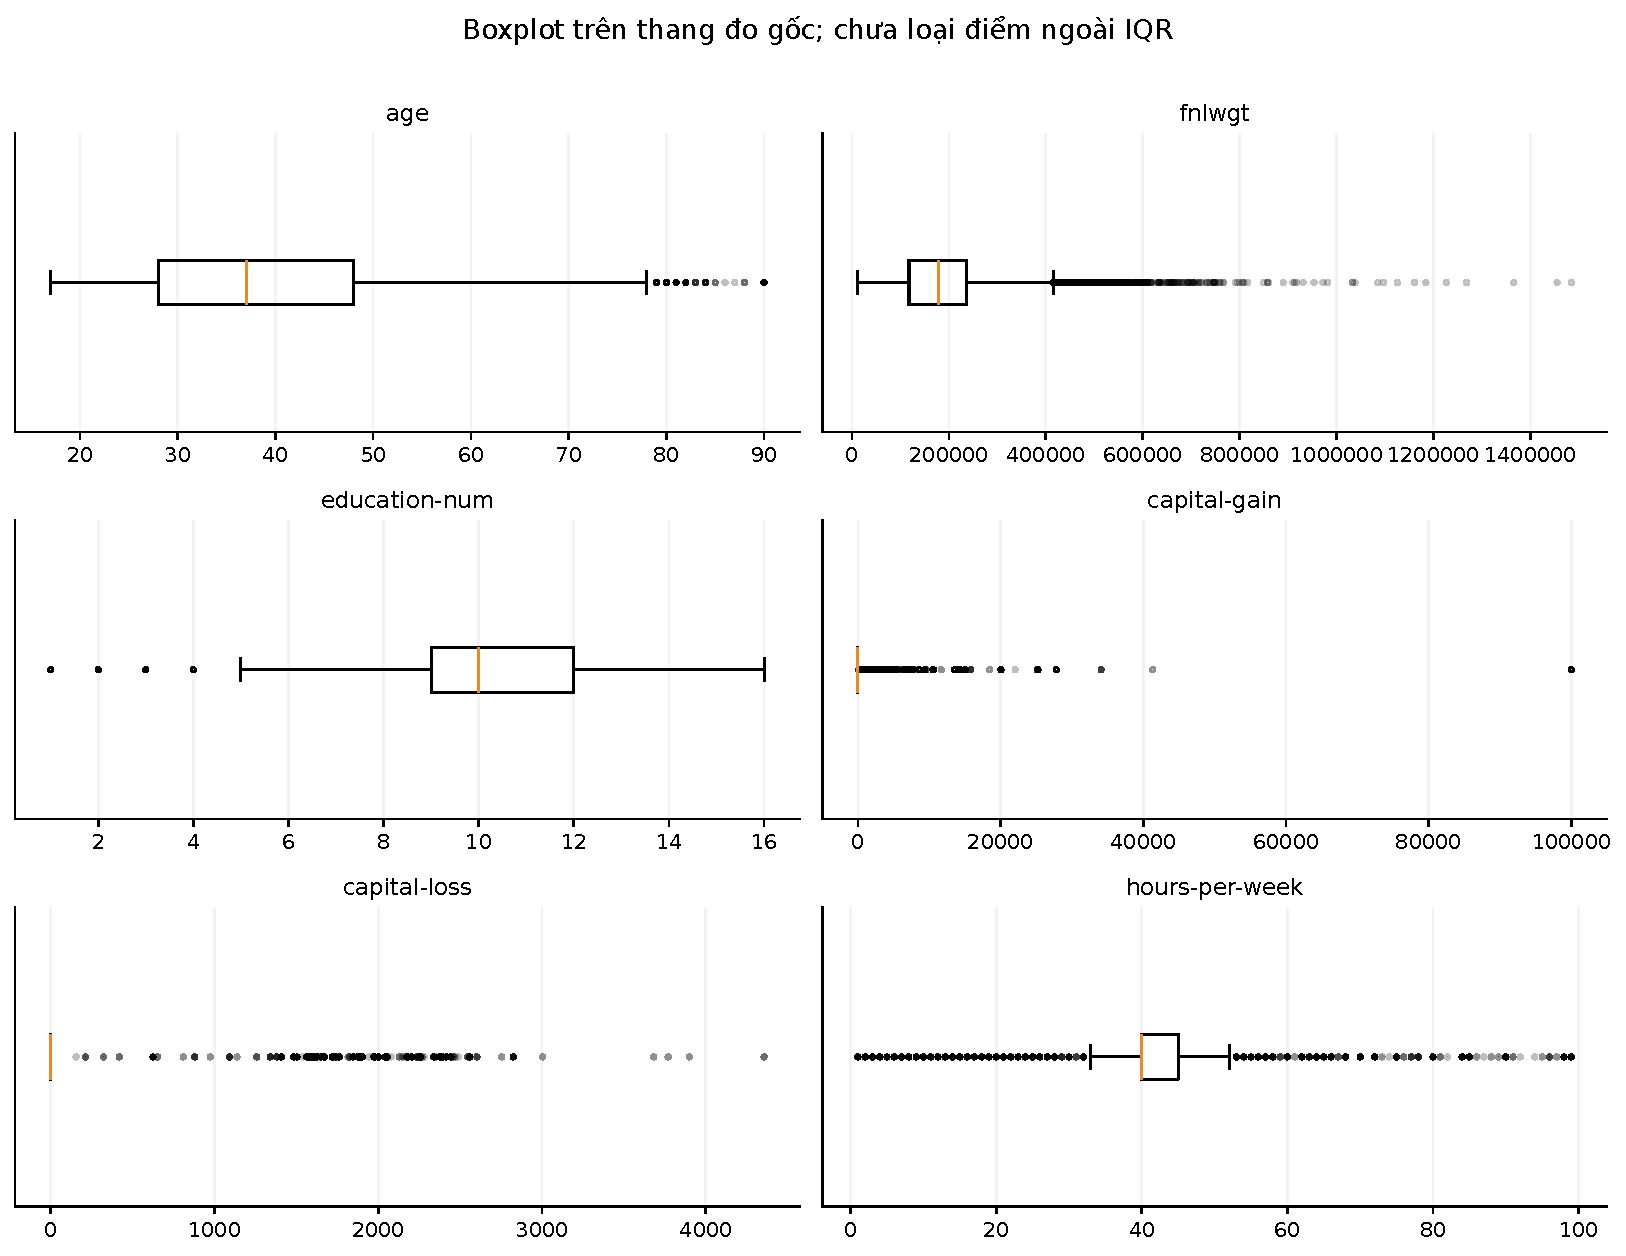
\includegraphics[width=.92\textwidth,height=.72\textheight,keepaspectratio]{Images/chapter_3/3_3/3_3_3/numeric_boxplots.pdf}
\caption{Boxplot riêng cho từng thuộc tính số trên thang đo gốc}
\label{fig:numeric-boxplots}
\end{figure}
